\documentclass[12pt, oneside]{memoir}

\newlength{\pagew}
\newlength{\pageh}
\setlength{\pagew}{210mm}
\setlength{\pageh}{297mm}

\setstocksize{\pageh}{\pagew}
\settrimmedsize{\pageh}{\pagew}{*}
\settypeblocksize{250mm}{150mm}{*}
\setlrmargins{*}{*}{1}
\setulmargins{*}{*}{1}
\setmarginnotes{0cm}{0cm}{0cm}
\checkandfixthelayout

% \usepackage[pass, showframe]{geometry}

\usepackage{mathpazo}
\usepackage{tgpagella}
\usepackage[T1]{fontenc}
\usepackage[mathscr]{eucal}

\usepackage{mathtools}
\usepackage{amsmath}
\usepackage{amsthm}

\usepackage{float}
\usepackage{graphicx}
\usepackage{svg}

\usepackage{enumitem}
\usepackage{tabto}
\usepackage{lipsum}

\usepackage{pst-solides3d}
\psset
{
  lightsrc=viewpoint,
  Decran=30,
  solidmemory,
}

\usepackage{tikz}
\usetikzlibrary{intersections}

\usepackage[
backend=biber,
style=alphabetic
]{biblatex}
\addbibresource{main.bib}

\usepackage[
colorlinks
]{hyperref}

\counterwithout{figure}{chapter}
\maxtocdepth{subsection}

\newtheorem{thm}{Théorème}
\newtheorem{prop}{Proposition}
\theoremstyle{definition}
\newtheorem{defn}{Définition}

% Unbutton the vector space from its origin.
\newcommand{\unbutton}[1][.6]{\mathbin{\vcenter{\hbox{\scalebox{#1}{$\bullet$}}}}}

% Definitional equal.
\newcommand{\defeq}{\vcentcolon=}

% Explicit set and set comprehension.
\newcommand{\set}[1]{\{ #1 \}}
\newcommand{\setcomp}[2]{\set{ #1 \,|\, #2 }}

% Projectivization.
\newcommand{\proj}{\boldsymbol{\mathscr{P}}}

% Disjoint union.
\newcommand{\discup}{\mathop{\dot{\cup}}}

% Partial map.
\newcommand*{\DashedArrow}[1][]{\mathbin{\tikz [baseline=-0.25ex,-latex, dashed,#1] \draw [#1] (0pt,0.5ex) -- (1.3em,0.5ex);}}%
\newcommand{\partialto}{\DashedArrow[->,dash pattern=on 4pt off 2pt]}

% Kernel and domain.
\DeclareMathOperator{\kernel}{Ker}
\DeclareMathOperator{\domain}{Dom}

% common sets
\newcommand{\R}{\mathbb{R}}

\begin{document}
\thispagestyle{empty}
\begin{center}
  \vspace*{\fill}
  % {%
  % \setlength{\fboxsep}{0pt}%
  % \fbox{\includesvg[width=3cm]{logo.svg}}%
  % }
  \includesvg[width=2.5cm]{logo.svg}

  \vspace{1cm}
  \large{\textbf{PROJET DE FIN D'ÉTUDES}}

  \vspace{0.5cm}
  {\small pour obtenir le diplôme de}

  \vspace{0.5cm}
  l'\textsc{\textbf{Université Galatasaray}}

  {\small Spécialité : \textbf{Mathématiques}}

  \vspace{2.25cm}
  {\Large\textbf{Formalisation du théorème de Desargue en Lean 4}}

  Rapport 1

  \vspace{1.25cm}
  Préparé par \textbf{Abdullah Uyu}

  Résponsable : \textbf{Can Ozan Oğuz}

  \vspace{2.25cm}
  \textit{5 novembre 2023}
  \vspace*{\fill}
\end{center}
\clearpage
\pagenumbering{arabic}
\section*{Introduction}
Lean 4 est un assistant de preuve. La transcription d'une preuve en
langage humain dans un assistant de preuve est appelée
\textit{formalisation}. Lean 4 dispose d'une grande bibliothèque de
preuves, y compris de nombreuses preuves du niveau de licence, appelée
mathlib4. Dans cette bibliothèque, il y a d'importants théorèmes
manquants, et le théorème de Desargue est l'un d'entre eux.
\section*{Objectifs du Projet}
Les deux aspects principaux de ce projet sont l'apprentissage des
rudiments de la théorie des géométries projectives, et de la
programmation en Lean 4. Avec ces deux aspects, le but ultime est de
formaliser le théorème de Desargue dans Lean 4.
\section*{Résultats Préliminaires}
Pour motiver les géométries projectives, on commence par considérer
les droites passant par l'origine dans le plan. On peut représenter la
plupart de ces lignes par des points sur l'axe $y=1$.
\begin{figure}[H]
  \centering
  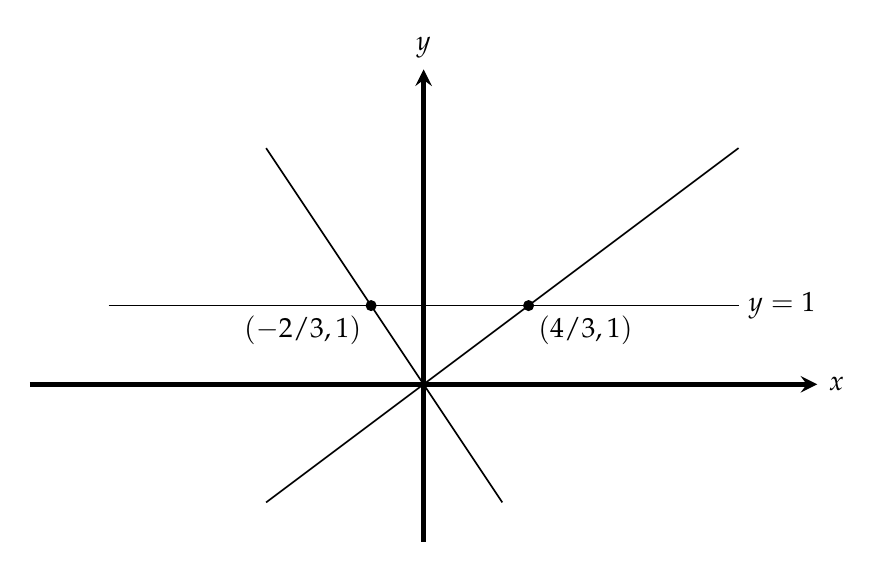
\begin{tikzpicture}
    \draw[-stealth,ultra thick] (-5,0)--(5,0) node[right] {$x$};
    \draw[-stealth,ultra thick] (0,-2)--(0,4) node[above] {$y$};
    \draw[name path=y1,semithick] (-4,1)--(4,1) node[right] {$y=1$};
    \draw[name path=line 1,semithick] (1,-1.5)--(-2,3) {};
    \draw[name path=line 2, semithick] (-2,-1.5)--(4,3) {};
    \fill[name intersections={of=y1 and line 1}] (intersection-1) circle (2pt)
    node[below left] {$(-2/3,1)$};
    \fill[name intersections={of=y1 and line 2}] (intersection-1) circle (2pt)
    node[below right] {$(4/3, 1)$};
  \end{tikzpicture}
  \caption{La représentation des droites passant par l'origine dans le
    plan}
  \label{fig:lines-plane}
\end{figure}
La seule droite que l'on n'a pas réussi à représenter est l'axe
$x$. On notera également que l'on peut bien sûr choisir n'importe quel
axe pour la représentation, à l'exception de ceux qui passent par
l'origine. Cette impossibilité dans les cas d'exception est clairement
visible sur la \autoref{fig:lines-plane}. Si l'on choisit un tel axe,
la droite que l'on ne parviendra pas à représenter sera la droite
(passant par l'origine) qui est parallèle à cet axe.

Effectuons la même procédure pour l'espace. On peut représenter la
plupart des droites passant par l'origine par des points sur le plan
$z=1$.
\begin{figure}[H]
  \centering
  \begin{pspicture}[viewpoint=30 40 30 rtp2xyz] (-5,-2) (5,4)
    \psSolid[object=plan,
    definition=equation,
    args={[0 0 1 0]},
    base=-2 3 -2 2.5]
    \psSolid[object=plan,
    definition=equation,
    args={[0 0 1 -2]},
    base=-2 3 -2 2.5]
    \psSolid[object=point,
    args=0 0 2]
    \psSolid[object=line,
    linestyle=dashed,
    args=0 0 0 -1 0.67 2]
    \psSolid[object=line,
    args=-1 0.67 2 -1.5 1 3]
    \psSolid[object=point,
    args=-1 0.67 2]
    \psSolid[object=line,
    linestyle=dashed,
    args=0 0 0 0.67 -1 2]
    \psSolid[object=line,
    args=0.67 -1 2 1 -1.5 3]
    \psSolid[object=point,
    args=0.67 -1 2]
    \axesIIID[labelsep=10pt] (0.5,0.5,2) (3.5,3.5,3.5)
    \rput(-2,3.05){$(-1/2,1/3,1)$}
    \rput(2.5,3.2){$(1/3,-1/2,1)$}
    \rput(3,1){$z=1$}
  \end{pspicture}
  \caption{La représentation des droites passant par l'origine dans l'espace}
  \label{fig:lines-space}
\end{figure}
Maintenant, les seules droites que nous ne pouvons pas représenter
sont exactement les droites du plan que nous avons représenté
précédemment. La remarque sur le choix de l'axe de représentation
s'étend ici comme tout plan ne passant pas par l'origine peut être
utilisé. De plus, le plan irreprésentable sera celui (qui passe par
l'origine) qui est parallèle au plan de représentation.

Ce processus s'appelle la \textit{projectivisation d'un espace
  vectoriel}. Écrivons-le en langage d'algèbre linéaire.
\begin{defn}[{\cite[27]{ff00}}]
  Soit $V$ un espace vectoriel. Sur
  $V^{\unbutton} \defeq V \setminus \set{0}$, on définit une relation
  binaire comme suit : $x \sim y$ ssi $x, y$ sont linéairement
  indépendants. Comme ceci est une relation d'équivalence, l'ensemble
  quotient $\proj(V) \defeq V^{\unbutton} / {\sim}$ est bien
  défini. $\proj(V)$ est appelée la \textit{projectivisation de
    l'espace vectoriel $V$}.
\end{defn}
Pour simplifier le langage, nous aurons également besoin de la
définition de l'union disjointe.
\begin{defn}
  Soit $A$ et $B$ deux ensembles. L'union
  $(A \times \set{1}) \cup (B \times \set{0})$, noté $A \discup B$, est
  appelée \textit{union disjointe} de $A$ et $B$.
\end{defn}
La motivation ci-dessus peut donc être formulée comme suit :
\begin{align*}
  \label{eq:embedding}
  \proj(\R^3) &= \proj(\R^2 \times \R) \\
              &\cong \R^2 \discup \proj(\R^2) \\
              &= \R^2 \discup \proj(\R \times \R) \\
              &\cong \R^2 \discup \R \discup \proj(\R)
\end{align*}
Cela résume ce que l'on fait mathématiquement lorsque l'on fait des
dessins en perspective : On prend un plan ($\R^2$), on choisit un
horizon ($\R$) et un point de fuite ($\proj(\R)$). La proposition
suivante n'est qu'une généralisation de ce processus.
\begin{prop}[{\cite[28]{ff00}}]
  Pour un $K$-espace vectoriel $V$, il existe une bijection naturelle
  \begin{equation*}
    \label{natural-bijection}
    s: \proj(V \times K) \to V \discup \proj(V)
  \end{equation*}
  induite par la fonction
  $t: (V \times K)^{\unbutton} \to V \discup \proj(V)$ définie par
  $t(x,\xi) = \xi^{-1}x$ if $\xi \neq 0$ et $t(x,0) = [x]$ pour
  $x \neq 0$, où $[x]$ désigne le point de $\proj(V)$ représenté par
  $x$.
  % Il existe donc une relation ternaire unique $\overline{\ell}$ sur
  % $V \discup \proj(V)$ pour laquelle $V \discup \proj(V)$ devient une
  % géométrie projective et $s$ un isomorphisme. De plus, on a:
  % \NumTabs{2}
  % \begin{enumerate}[align=left]
  % \item $\overline{\ell}(x, y, z)$ \tabto{3cm} ssi $x-z$ et $y-z$ sont linéairement
  %   dépendants dans $V$,
  % \item $\overline{\ell}(x, y, [z])$ \tabto{3cm} ssi $x-y = \mu z$ pour un $\mu \in
  %   K$
  % \item $\overline{\ell}(x, [y], [z])$ \tabto{3cm} ssi $[y] = [z]$,
  % \item $\overline{\ell}([x], [y], [z])$ \tabto{3cm} ssi $\ell([x], [y], [z])$.
  % \end{enumerate}
\end{prop}

\begin{defn}[{\cite[26]{ff00}}]
  Une \textit{géométrie projective} est un ensemble $G$ accompagné
  d'une relation ternaire $\ell \subseteq G \times G \times G$ telle
  que les axiomes suivants sont satisfaits :
  \begin{itemize}[align=left]
  \item[($\text{L}_1$)] $\ell(a,b,a)$ pour tout $a, b \in G$.
  \item[($\text{L}_2$)] $\ell(a,p,q)$, $\ell(b,p,q)$ et $p \neq q$
    $\implies$ $\ell(a,b,p)$.
  \item[($\text{L}_3$)] $\ell(p,a,b)$ et $\ell(p,c,d)$ $\implies$
    $\ell(q,a,c)$ et $\ell(q,b,d)$ pour un $q \in G$.
  \end{itemize}
  Les éléments de $G$ sont appelés les \textit{points} de la
  géométrie. Et trois points $a, b, c$ sont dits \textit{colinéaires}
  si $\ell(a,b,c)$.
\end{defn}
% Un système équivalent d'axiomes utilisant l'ensemble, par exemple,
% $a \star b$, créé par $\ell$ est omis ici, par souci de concision. La
% définition de morphisme sera donnée à l'aide de ce système.

Notons l'exemple le plus important pour une géométrie projective. Lors
d'une discussion sur la chaîne de Zulip de Lean 4, Joseph Myers a
conseillé d'énoncer le théorème sur cet exemple, mais pas sur la
définition abstraite d'une géométrie projective. De plus, il est noté
que la version du théorème en géométrie euclidienne, qui est
probablement même connue de nombreux élèves du lycée, peut être
déduite de l'énoncé du théorème sur cet important modèle de géométrie
projective.
\begin{prop}[{\cite[27]{ff00}}]
  Pour un espace vectoriel $V$, $\proj(V)$ est une géométrie
  projective si pour tout élément $X, Y, Z \in \proj(V)$ on définit :
  $\ell(X,Y,Z)$ ssi $X, Y, Z$ ont des représentants $x, y, z$
  linéairement dépendants.
\end{prop}
Notons maintenant la définition d'un isomorphisme de géométries
projectives et une proposition d'isomorphisme.
\begin{defn}[{\cite[27]{ff00}}]
  Un \textit{isomorphisme} de géométries projectives est une bijection
  $g: G_1 \to G_2$ satisfaisant $\ell_1(a,b,c)$ ssi
  $\ell_2(ga,gb,gc)$. Si $G_1 = G_2$, alors on dit que $g$ est une
  \textit{collinéation}.
\end{defn}
% Pour arriver à définir les endomorphisms, on note les définitions de
% fonction partielle, de noyau et domaine d'un fonction partielle, de
% sous-espace d'un géométrie projective, de morphisme et d'hyperplan.
% \begin{defn}
%   Une \textit{fonction partielle} de $X$ dans $Y$ est une fonction
%   $f: X \setminus N \to Y$ définie sur le complément d'un
%   sous-ensemble $N \subseteq X$. Si $f$ est une fonction partielle de
%   $X$ dans $Y$, on écrit $f: X \partialto Y$, ou encore $f: X \to Y$
%   si on sait que $N = \emptyset$. L'ensemble $N$ est appelé
%   \textit{noyau} de $f$ et sera désigné par $\kernel f$. L'ensemble
%   $X \setminus N$ est appelé \textit{domaine} de $f$ et sera désigné
%   par $\domain f$.
% \end{defn}
% \begin{defn}
%   Un \textit{sous-espace} d'un géométrie projective $G$ est un sous-ensemble $E
%   \subseteq G$ satisfaisant :
%   \begin{equation*}
%     \label{subspace}
%     a,b \in E \implies a \star b \subseteq E
%   \end{equation*}
% \end{defn}
% \begin{defn}
%   Un \textit{morphisme} d'un géométrie projective $G_1$ dans un
%   géométrie projective $G_2$ est une fonction partielle $g: G_1
%   \partialto G_2$ satisfaisant les axiomes suivant :
%   \begin{itemize}[align=left]
%   \item[($\text{M}_1$)] $\kernel g$ est un sous-espace de $G_1$,
%   \item[($\text{M}_2$)] si $a, b \not\in N$, $c \in N$ et $a \in b
%     \star c$, alors $ga = gb$,
%   \item[($\text{M}_3$)] si $a, b, c \not\in N$ et $a \in b \star c$,
%     alors $ga \in gb \star gc$.
%   \end{itemize}
% \end{defn}
% \begin{defn}
%   Un \textit{hyperplan} d'une géométrie projective $G$ est un
%   sous-espace $H$ de $G$ qui est maximal parmi les sous-espaces
%   stricts de $G$.
% \end{defn}
% Nous définissons enfin les endomorphismes, ainsi que le centre et
% l'axe d'un endomorphisme.
% \begin{defn}
%   Un \textit{endomorphisme} d'un géométrie projective $G$ est un
%   morphisme $\varphi: G \partialto G$. Un \textit{centre} d'un
%   endomorphisme $\varphi: G \partialto G$ est un point $z \in G$ tel
%   que $\varphi x \in x \star z$ pour tout $x \in \domain \varphi$. Un
%   \textit{axe} d'un endomorphisme $\varphi: G \partialto G$ est un
%   hyperplan $H \subseteq G$ tel que $\varphi x = x$ pour tout $x \in H
%   \cap \domain \varphi$.
% \end{defn}
\section*{Prochaines Étapes}
Tout d'abord, la preuve en langage humain du théorème sera
minutieusement assimilée. Pour cela, le livre "Modern Projective
Geometry" \cite{ff00} de Claude-Alain Faure et Alfred Frölicher sera
utilisé. Ce livre offre un cadre complet pour l'étude des géométries
projectives. En particulier, le théorème de Desargue est compris en
termes d'endomorphismes des géométries projectives et la preuve est
effectuée en conséquence.

Deuxièmement, l'existence des transcriptions de la machinerie requise,
dans mathlib4 sera vérifiée. Quelques exemples seraient la définition
de la projectivisation, des morphismes entre des espaces projectifs,
etc.

Enfin, le schéma complet de la preuve sera transcrit. Cela nécessitera
probablement une bonne maîtrise de la programmation en Lean 4, et il
est prévu que cette exigence soit satisfaite en cours de route.
\nocite{*}
\printbibliography[title=Références,heading=subbibliography]
\end{document}
